\documentclass[journal]{IEEEtran}

\usepackage[utf8]{inputenc}
\usepackage{graphicx}
\usepackage{verbatim}
\usepackage{color}
\usepackage{xcolor}
\usepackage{xspace}

\graphicspath{{figs/}}

\newcommand{\fsk}          {    FSK\_868}
\newcommand{\oqpsk}        {O-QPSK\_2.4}
\newcommand{\ofdm}         {OFDM\_868}

\newcommand{\todo}[1]      {\textbf{\textcolor{red}{[TODO] #1}}}
\newcommand{\lorem}        {\textcolor{green}{Lorem ipsum dolor sit amet, consectetur adipiscing elit, sed do eiusmod tempor incididunt ut labore et dolore magna aliqua. Ut enim ad minim veniam, quis nostrud exercitation ullamco laboris nisi ut aliquip ex ea commodo consequat. Duis aute irure dolor in reprehenderit in voluptate velit esse cillum dolore eu fugiat nulla pariatur. Excepteur sint occaecat cupidatat non proident, sunt in culpa qui officia deserunt mollit anim id est laborum.}}
\newcommand{\mina}[1]      {\textbf{\textcolor{blue}{[Mina] #1}}}
\newcommand{\quentin}[1]   {\textbf{\textcolor{blue}{[Quentin] #1}}}
\newcommand{\dominique}[1] {\textbf{\textcolor{blue}{[Dominique] #1}}}
\newcommand{\thomas}[1]    {\textbf{\textcolor{blue}{[Thomas] #1}}}

\begin{document}


\title{No Free Lunch?: 6TiSCH Performance\\on Different Modulations}

\author{
    \IEEEauthorblockN{
        Mina~Rady\IEEEauthorrefmark{1,2},
        Quentin~Lampin\IEEEauthorrefmark{1},
        Dominique~Barthel\IEEEauthorrefmark{2},
        Thomas~Watteyne\IEEEauthorrefmark{2}
    }\\
    \IEEEauthorblockA{
        \IEEEauthorrefmark{1}~Orange Labs, Meylan, France
    }\\
    \IEEEauthorblockA{
        \IEEEauthorrefmark{2}~EVA team, Inria, Paris, France
    }
    \thanks{Corresponding author: Mina~Rady (email: {\tt poipoi})}
}

\maketitle

\begin{abstract}
   \lorem
   \lorem
   \lorem
\end{abstract}

\tableofcontents

%==============================================================================
\section{Introduction}
\label{sec:introduction}

% intro low-power wireless

\lorem

% popular PHY layers

\lorem IEEE 802.15.4

% capabilites of recent chips

\lorem nRF52840, CC2538, CC2650

% goal

\lorem

% contributions
\mina {Updated Findings in a nutshell (for abstract?):}
\begin{itemize}

\item  \fsk is best fo fast network formation, least end-to-end latency, and least packet buffer memory footprint, but risks neighbor table overflow in dense deployments.

\item \oqpsk is worst for latency but best forneighbor discovery in dense deployments and for battery life time.
 
\item  \ofdm, even though it is the highest bitrate, it shows a comporomise between both radios. It falls in between both in terms of neighbor discovery range, battery lifetime, memory footprint, end-to-end latency. Despite its long range comparable to FSK, it has an overall low duty cycle comparable to OQPSK. And despite its high bitrate, it shows range capability comparable to FSK.
\end{itemize}

The contributions of this article are three-fold:

\begin{itemize}
   \item \todo{Using \fsk the most number of neighbors are discovered. It leads to the fastest network formation time with the highest latency and lower network depth.Yet it kills network battery lifetime. It risks neighbor table overflow in high density deployments.}
   \item \todo{Using \oqpsk, the least number of neighbors are discovered. It leads to the slowest network formation time, highest RPL depth (lowest DAG ranks) and effectively the highest end-to-end latency. It consumes the most packet buffer on average because of storage needed to retransmissions}
   \item \todo{Usig \ofdm, number of discovered neighbors is in between \fsk and \oqpsk, despite being the highest bitrate in the three modulations. It shows an intermeidate neighbor discovery range between both modulations. It shows surprisingly a network formation speed, and end-to-end latency comparable to \fsk. Yet it has a duty cycle comparable to OQPSK. It shows the least steady-state PDR among the three. }
\end{itemize}
  

% remainder

The remainder of this article is organized as follows.
Section~\ref{sec:opentested} \todo{}.

%==============================================================================
\section{The OpenTestbed}
\label{sec:opentested}

% intro testbed, architecture

\lorem

% OpenMote and testbox

\lorem

\begin{figure}
	\centering
	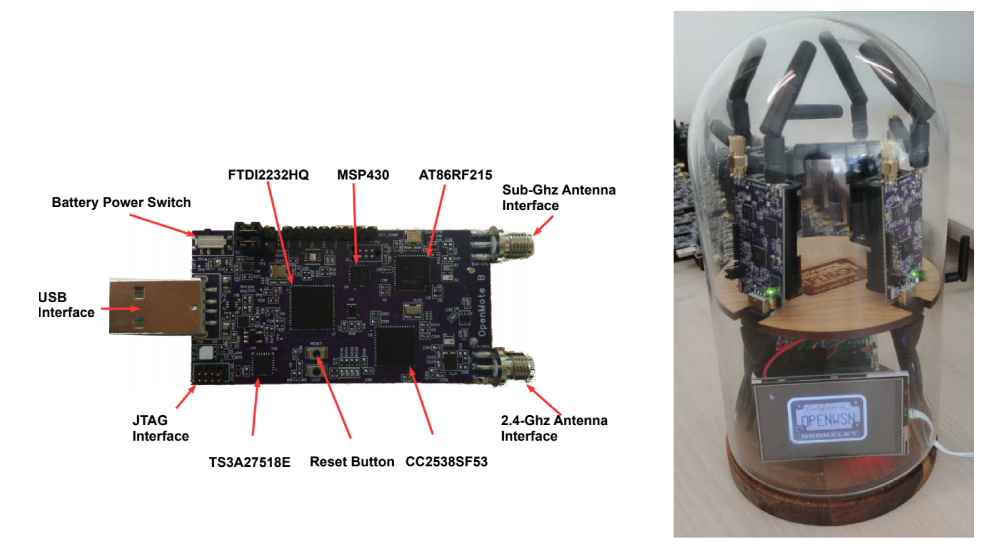
\includegraphics[width=0.90\columnwidth]{mote_ot}
	\caption{OpenMote B board (left) and The testbox containing four OpenMote B boards (right).}
    \label{fig:testbox}
\end{figure}

% 42-mote deployment

\lorem

\begin{figure}
	\centering
	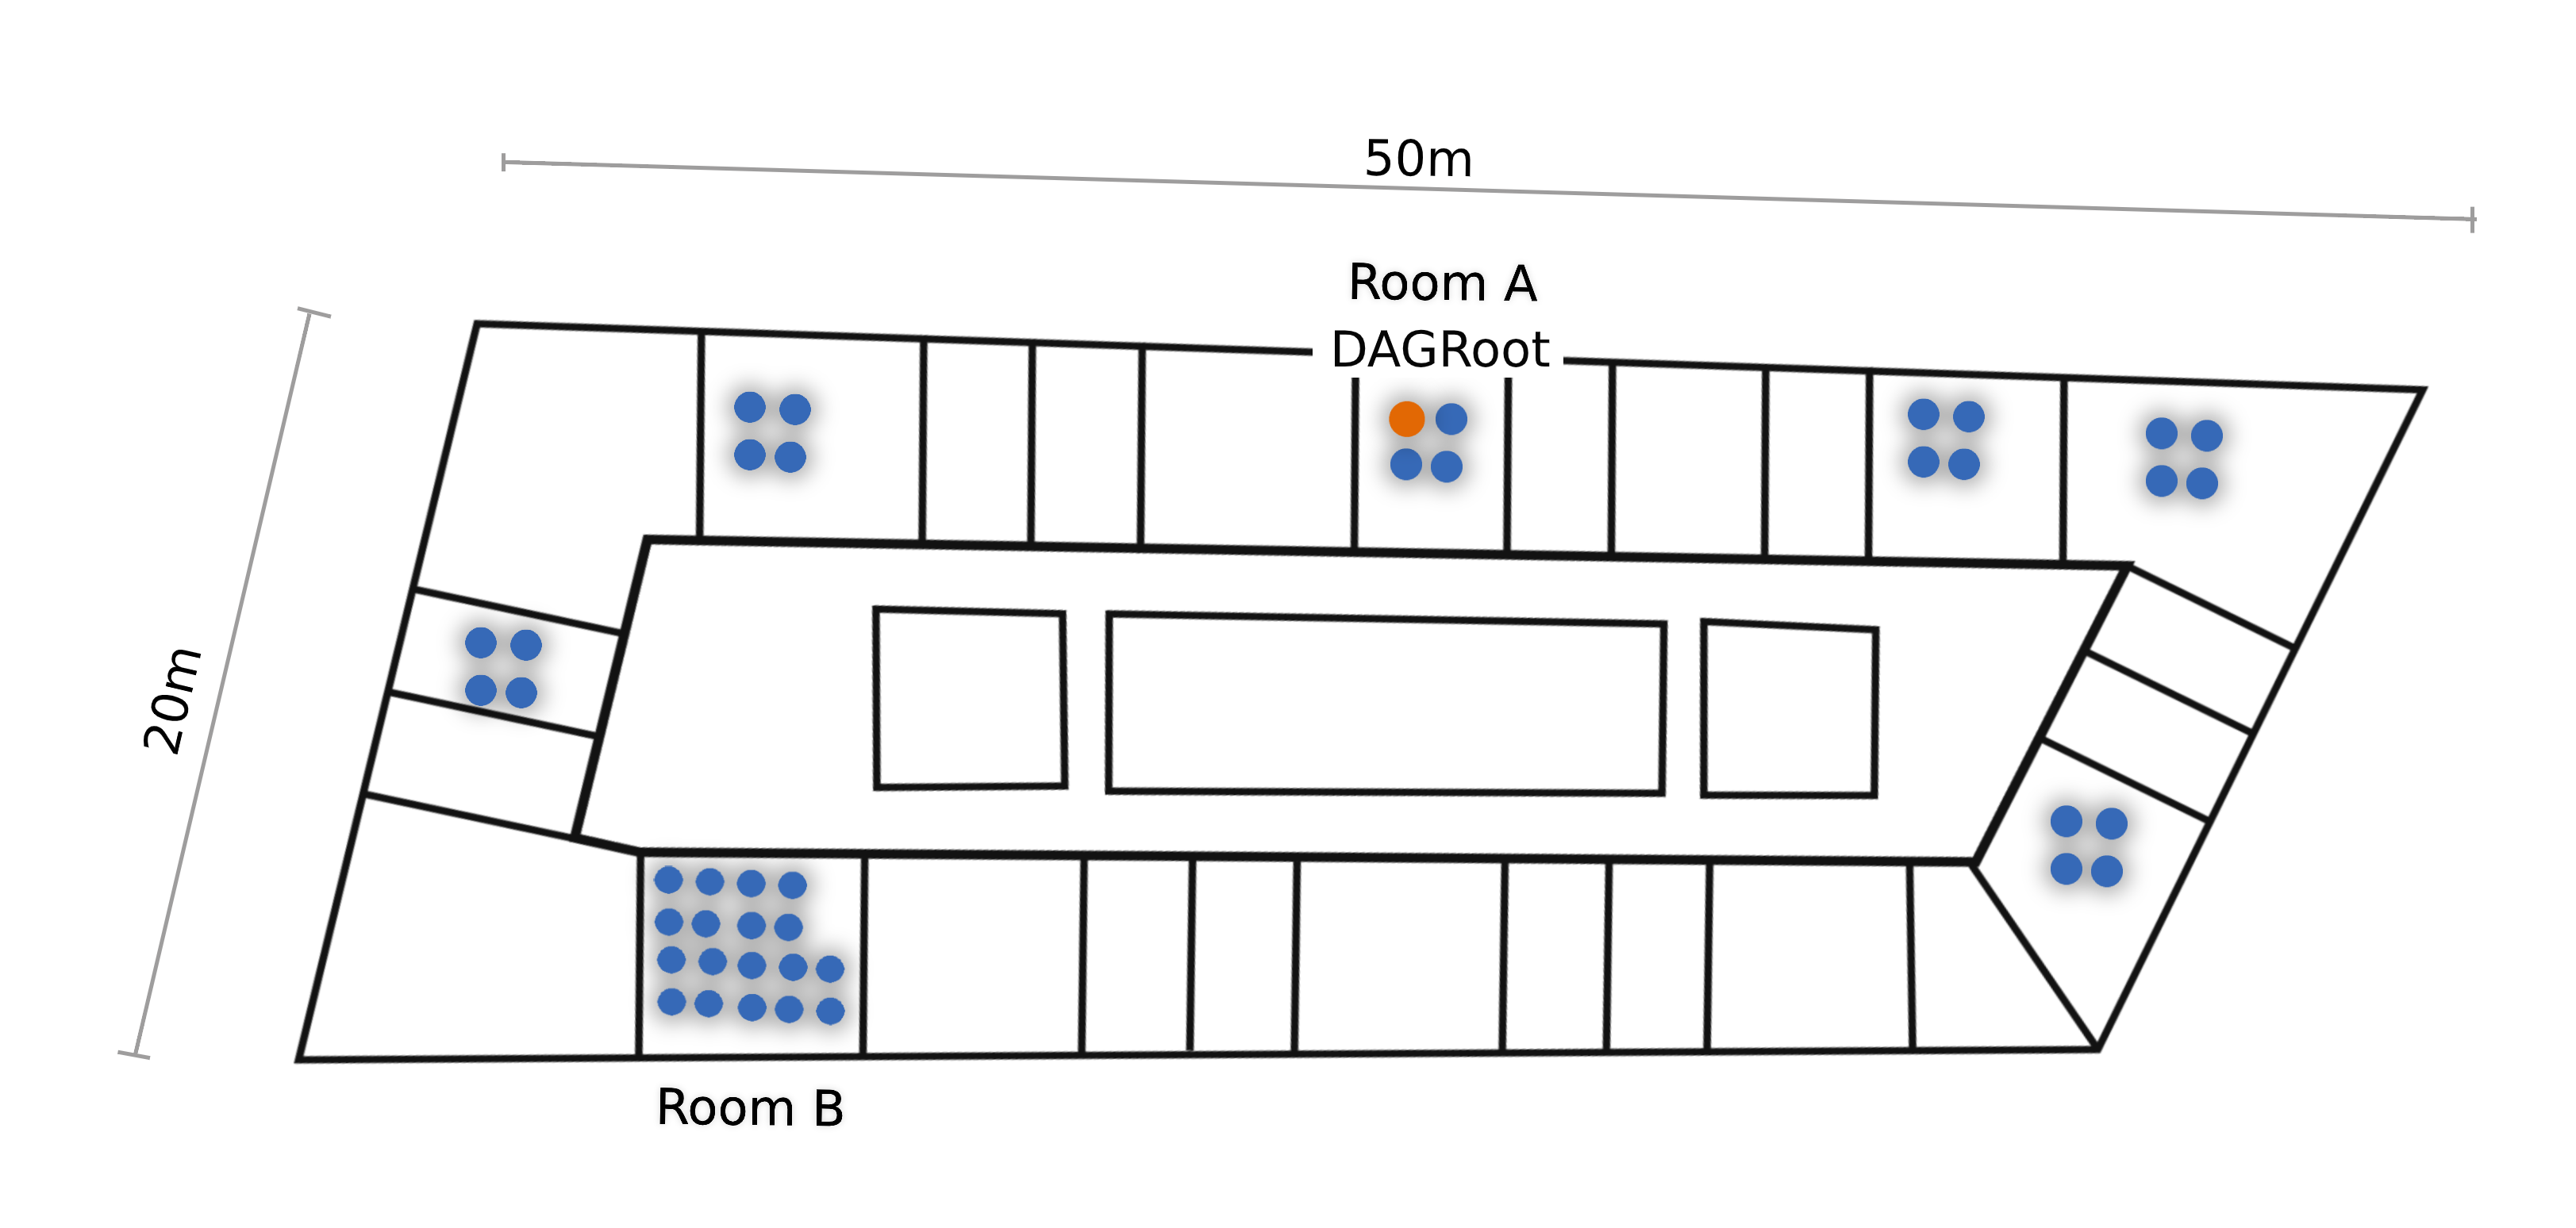
\includegraphics[width=0.90\columnwidth]{building_motes}
	\caption{Floorplan of the deployment.}
    \label{fig:floorplan}
\end{figure}

%==============================================================================
\section{An PHY-later Agile Extension of OpenWSN}
\label{sec:openwsn}

% intro to 6TiSCH

\lorem

% intro to OpenWSN

\lorem

% goal: multiple PHY layer

\lorem \fsk \oqpsk \ofdm``FSK\_subGHz''

% OpenWSN Extension

\lorem

% result: footprint

\lorem

%==============================================================================
\section{Methodology}
\label{sec:methodology}

% repeating 3 times

\lorem

% duration of one experiment

\lorem

% gathering data, publishing raw results, etc.

\lorem

% KPIs

\lorem

% running the experiments

\lorem

%==============================================================================
\section{Experimental Results}
\label{sec:results}

\lorem

%------------------------------------------------------------------------------
\subsection{Network Formation}
\label{sec:network_formation}

% why is it important, define

\lorem

% worst case from a contention point of view

\lorem

% results

\lorem Fig.~\ref{fig:time_firstpacket_cdf}

\begin{figure}
	\centering
	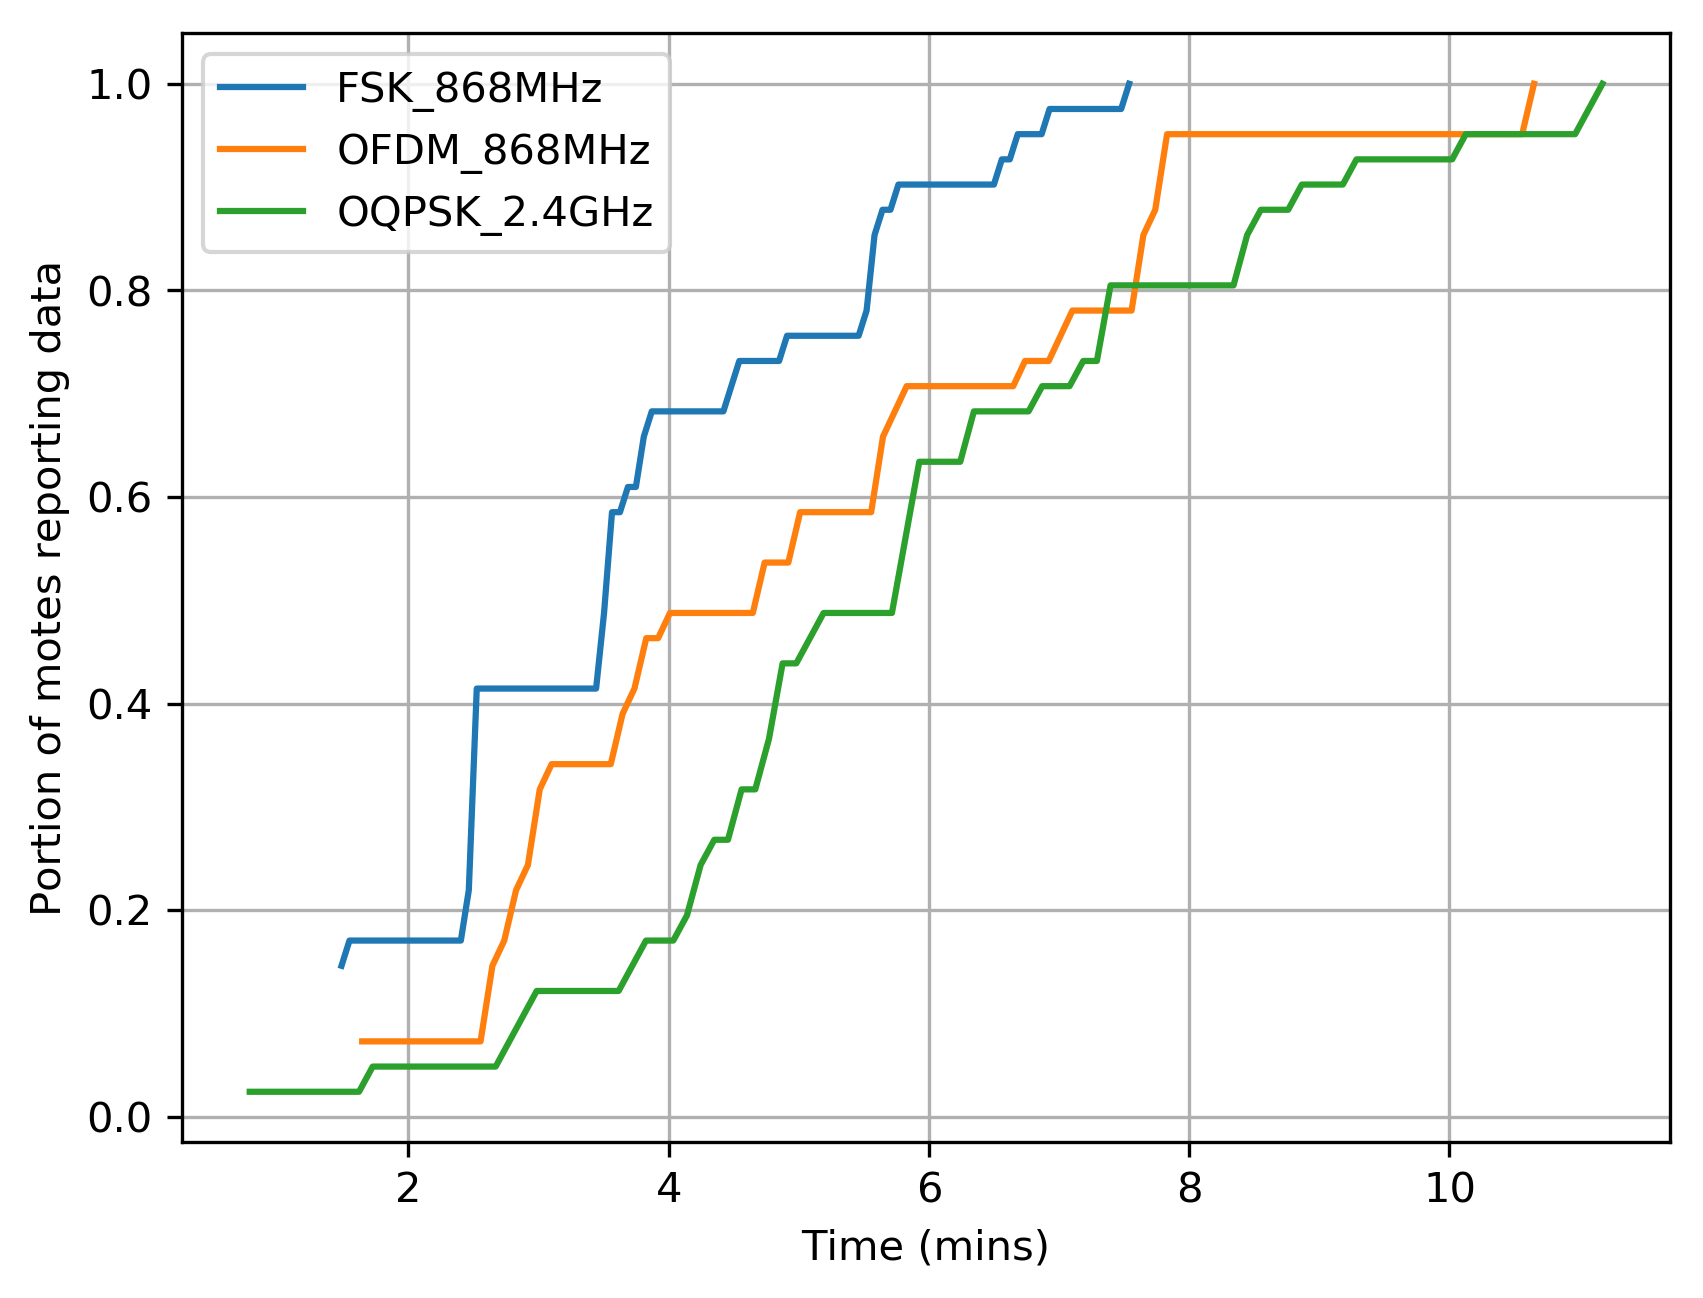
\includegraphics[width=0.90\columnwidth]{time_firstpacket_cdf}
	\caption{Time to First Packet CDF.}
    \label{fig:time_firstpacket_cdf}
\end{figure}

% settling time, steady-state   

\begin{figure}
	\centering
	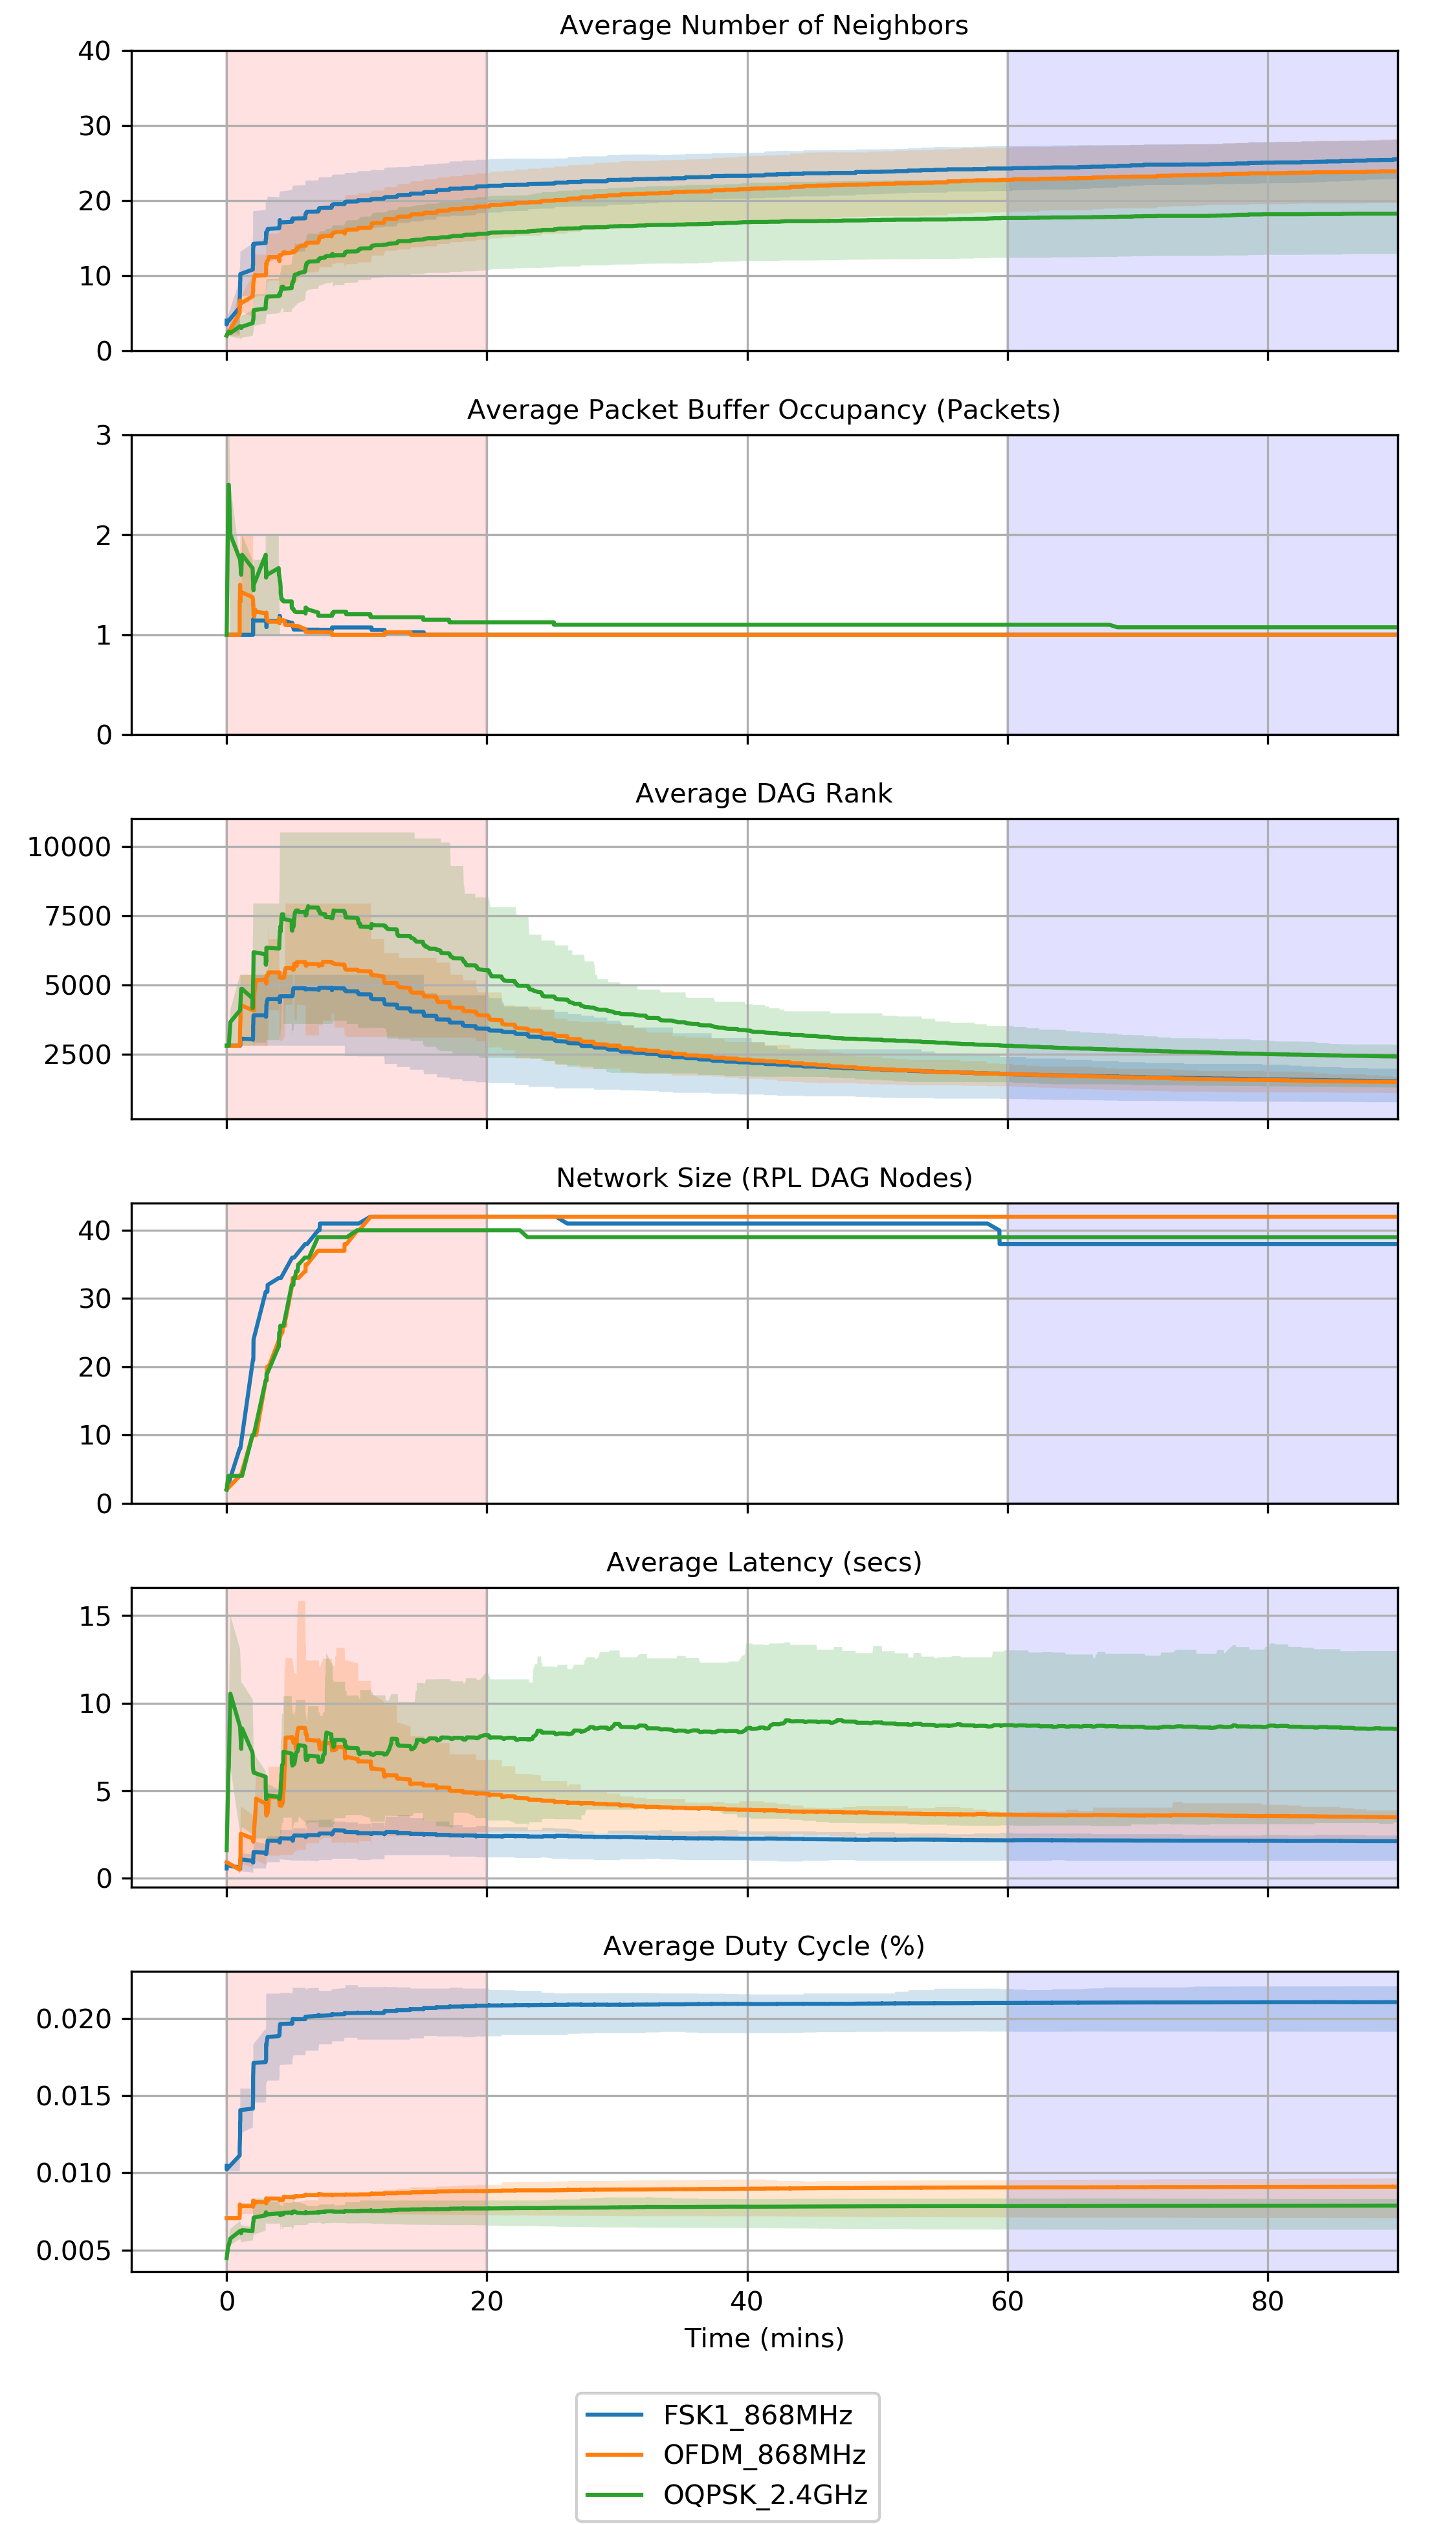
\includegraphics[width=0.90\columnwidth]{aggregate_plot_reliability}
	\caption{6TiSCH reliability performance under each radio setting in the three stages of network formation: 1) discovery and formation phase (red highlight),and 2) steady-state phase (blue highlight). Shaded curves represent the majority of the distribution (interquartile range)}
    \label{fig:aggregate_plot_reliability}
\end{figure}

%Network seems to be forming generalAlso combining the observations from the average network degree in Fig.~\ref{fig:avg_numNeighbors_plot} and average network depth in fig. \ref{fig:avg_dagRank_plot}, it can be observed that as the network grows, FSK seems show generally lower DAG rank on average in the network yet with generally higher network degree.

%ly faster using sub-GHz radio. This is reflected in CDF of time to first packet (Fig.~\ref{fig:time_firstpacket_cdf}) and in network size at routing layer (Fig. \ref{fig:rpl_node_count_plot}). 

%\begin{figure}
%	\centering
%	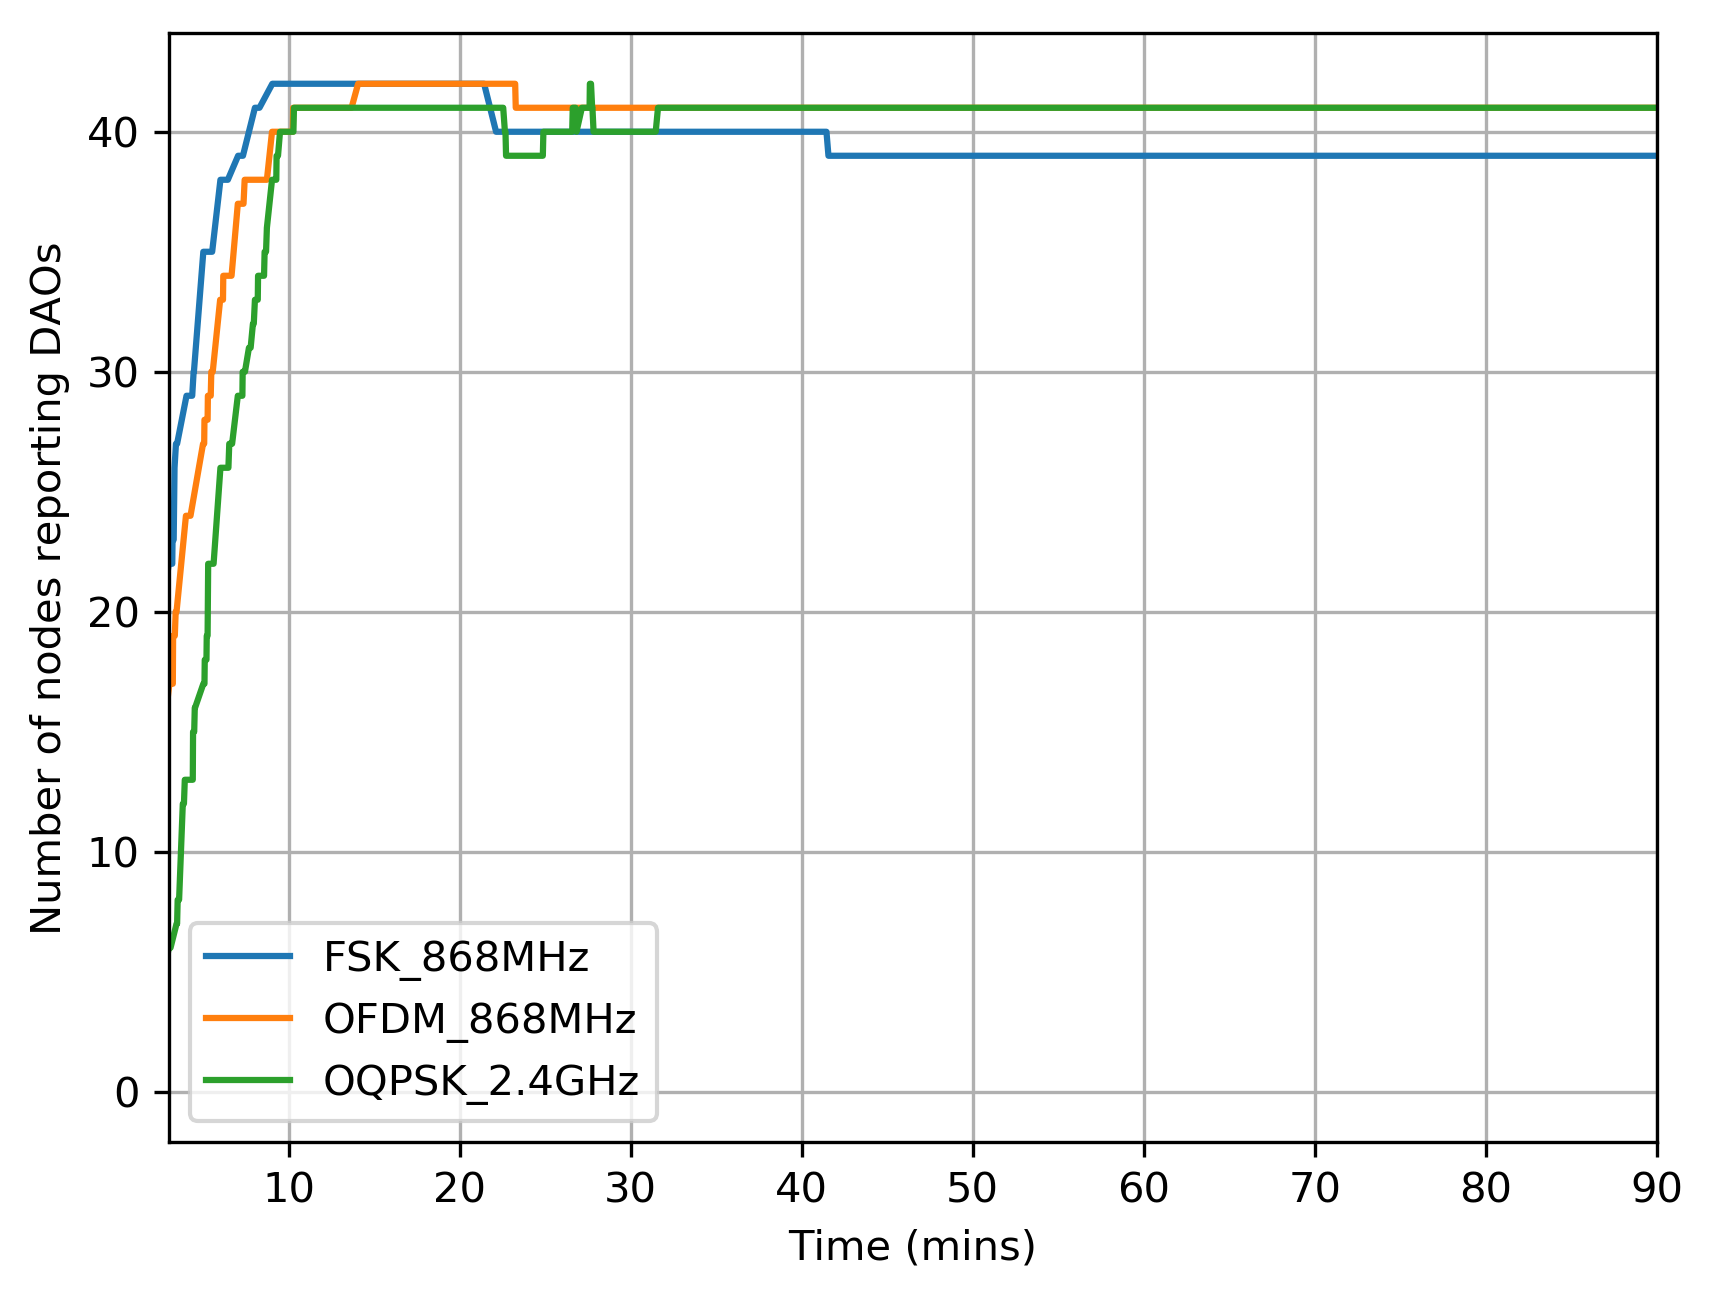
\includegraphics[width=0.90\columnwidth]{rpl_node_count_plot.png}
%	\caption{Network growth at routing layer}
%    \label{fig:rpl_node_count_plot}
%\end{figure}

%------------------------------------------------------------------------------
\subsection{End-to-End Reliability}
\label{sec:reliability}

Conclusion from fig. \ref{fig:aggregate_plot_reliability}: FSK leads to more neighbors heard at receiver on the minimum cell and faster overflow of the neighbor table.
The positive side is that motes have access to parents closer to the root with lower DAGRanks and therefore the average network depth is decreased. 
The negative side is that a mote becomes more likely to miss newer neighbors even though they could be with link higher quality. Therefore PDR becomes less-optimal. 



\begin{table}
 \caption {Steady-state end-to-end PDR values} \label{tab:pdr_table} 
 \begin{center}
 \begin{tabular}{||c c c c||} 
 \hline
 Radio Setting & Average & Median & Stdev \\ [0.5ex] 
 \hline\hline
 \fsk & 100\% & 100\% & 0 \\ 
 \hline
 \ofdm & 99,9521\% & 100\% & 0.302 \\
 \hline
 \oqpsk & 100\% & 100\% & 0 \\
 \hline

\end{tabular}
\end{center}
\end{table}


\begin{figure}
	\centering
	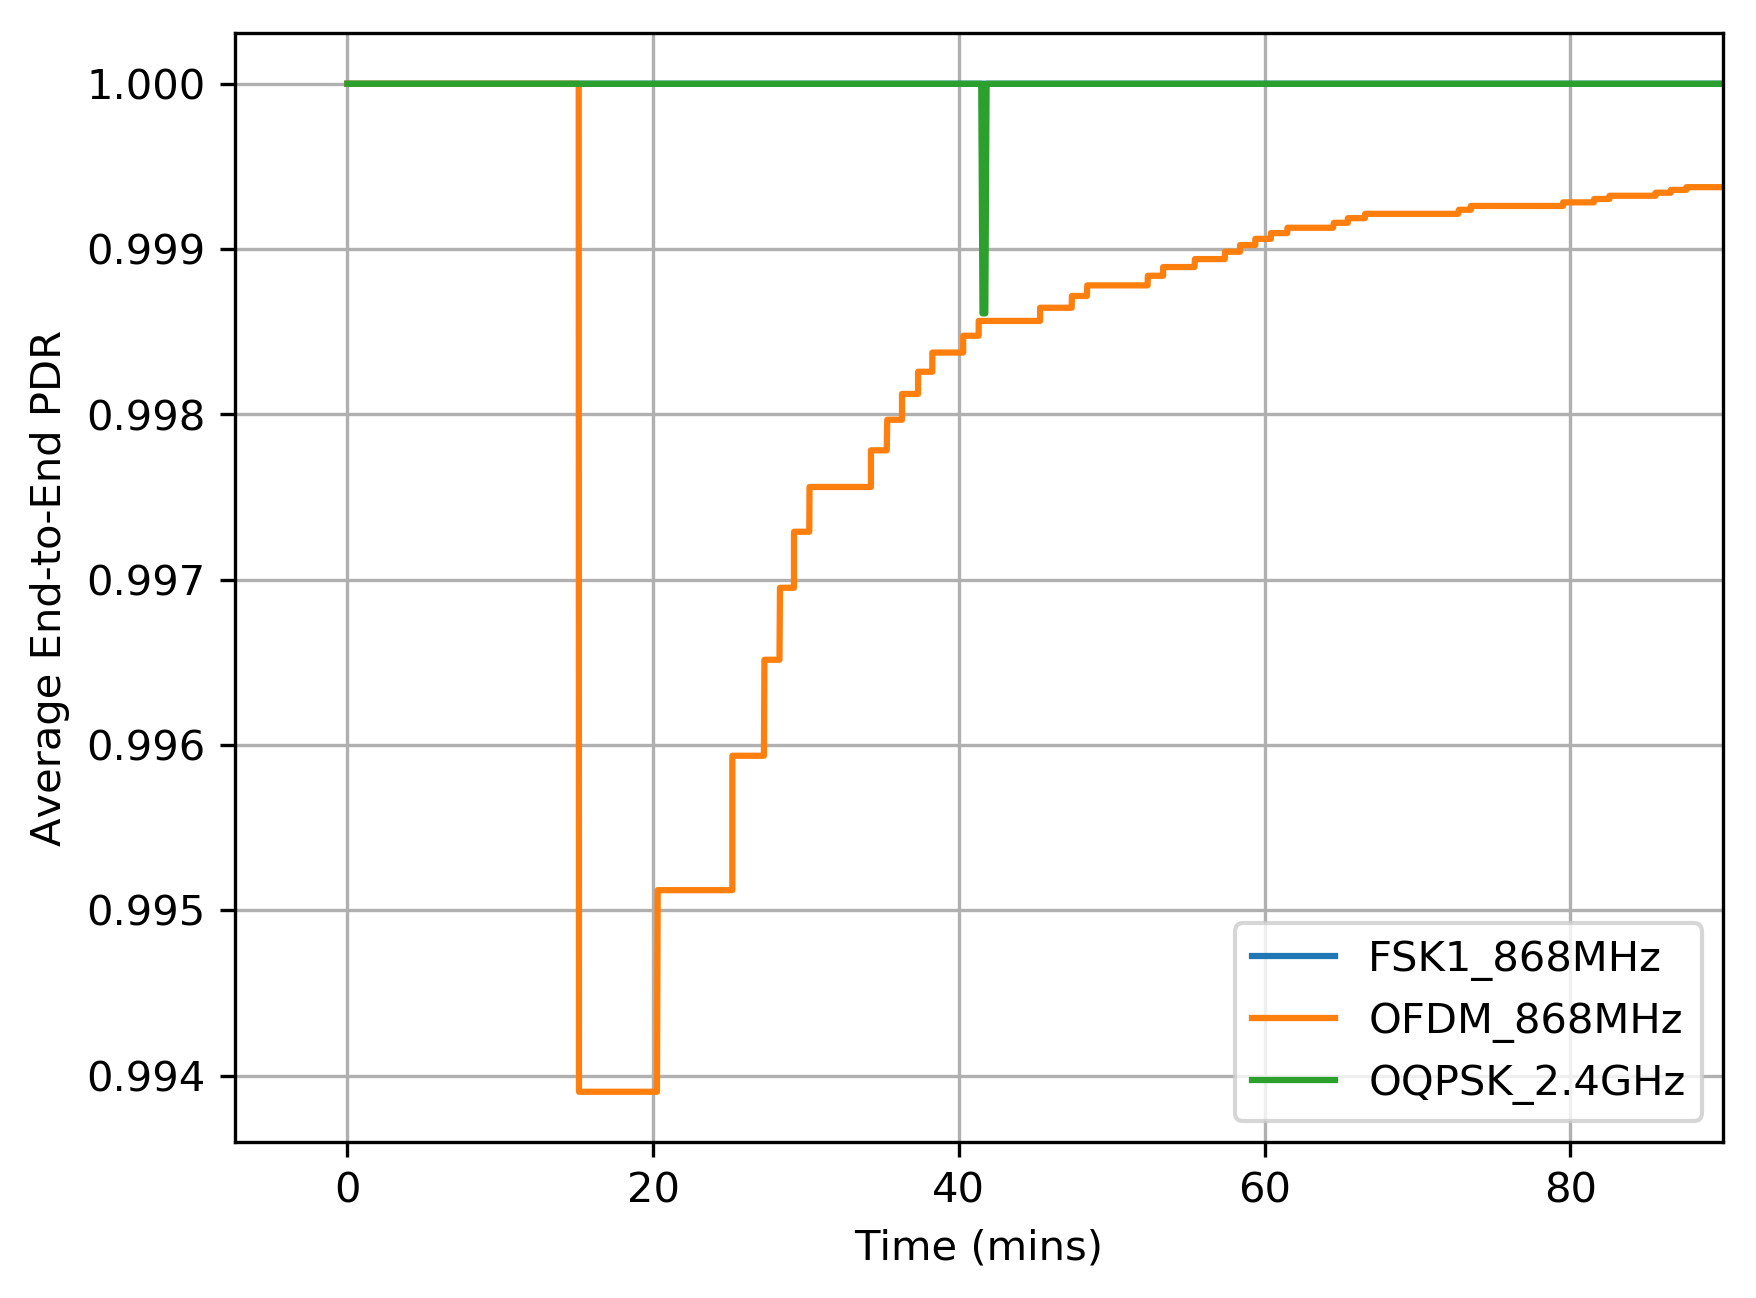
\includegraphics[width=0.9\columnwidth]{avg_pdr_plot.png}
	\caption{Average end-to-end PDR. }
    \label{fig:avg_pdr_plot}
\end{figure} 

%------------------------------------------------------------------------------
\subsection{End-to-End Latency}
\label{sec:latency}

The 6TiSCH stack on top of FSK demonstrates better end to end latency by 2 or 3 orders of magnitude than OFDM or OQPSK as observed in Fig.~\ref{fig:avg_latency_plot}.
\dominique{a factor 2 or 3, not 2 or 3 orders of magnitude!!}
The interquartile range in the same figure show generally homogeneous latency properties in the FSK-based mesh. 
However as shorter range radios are utilized, it seems that a minority of nodes suffer from very high latency, skewing the average latency in the network far away from the interquartile range. 
This could imply a generally unstable QOS expectation in the networks based on OFDM and OQPSK despite their high reliability as previously seen in Fig.~\ref{fig:avg_pdr_plot}. 
This could be caused by the larger number of nodes with higher DAG ranks (i.e. with more hops away from the root).

\begin{figure}
	\centering
	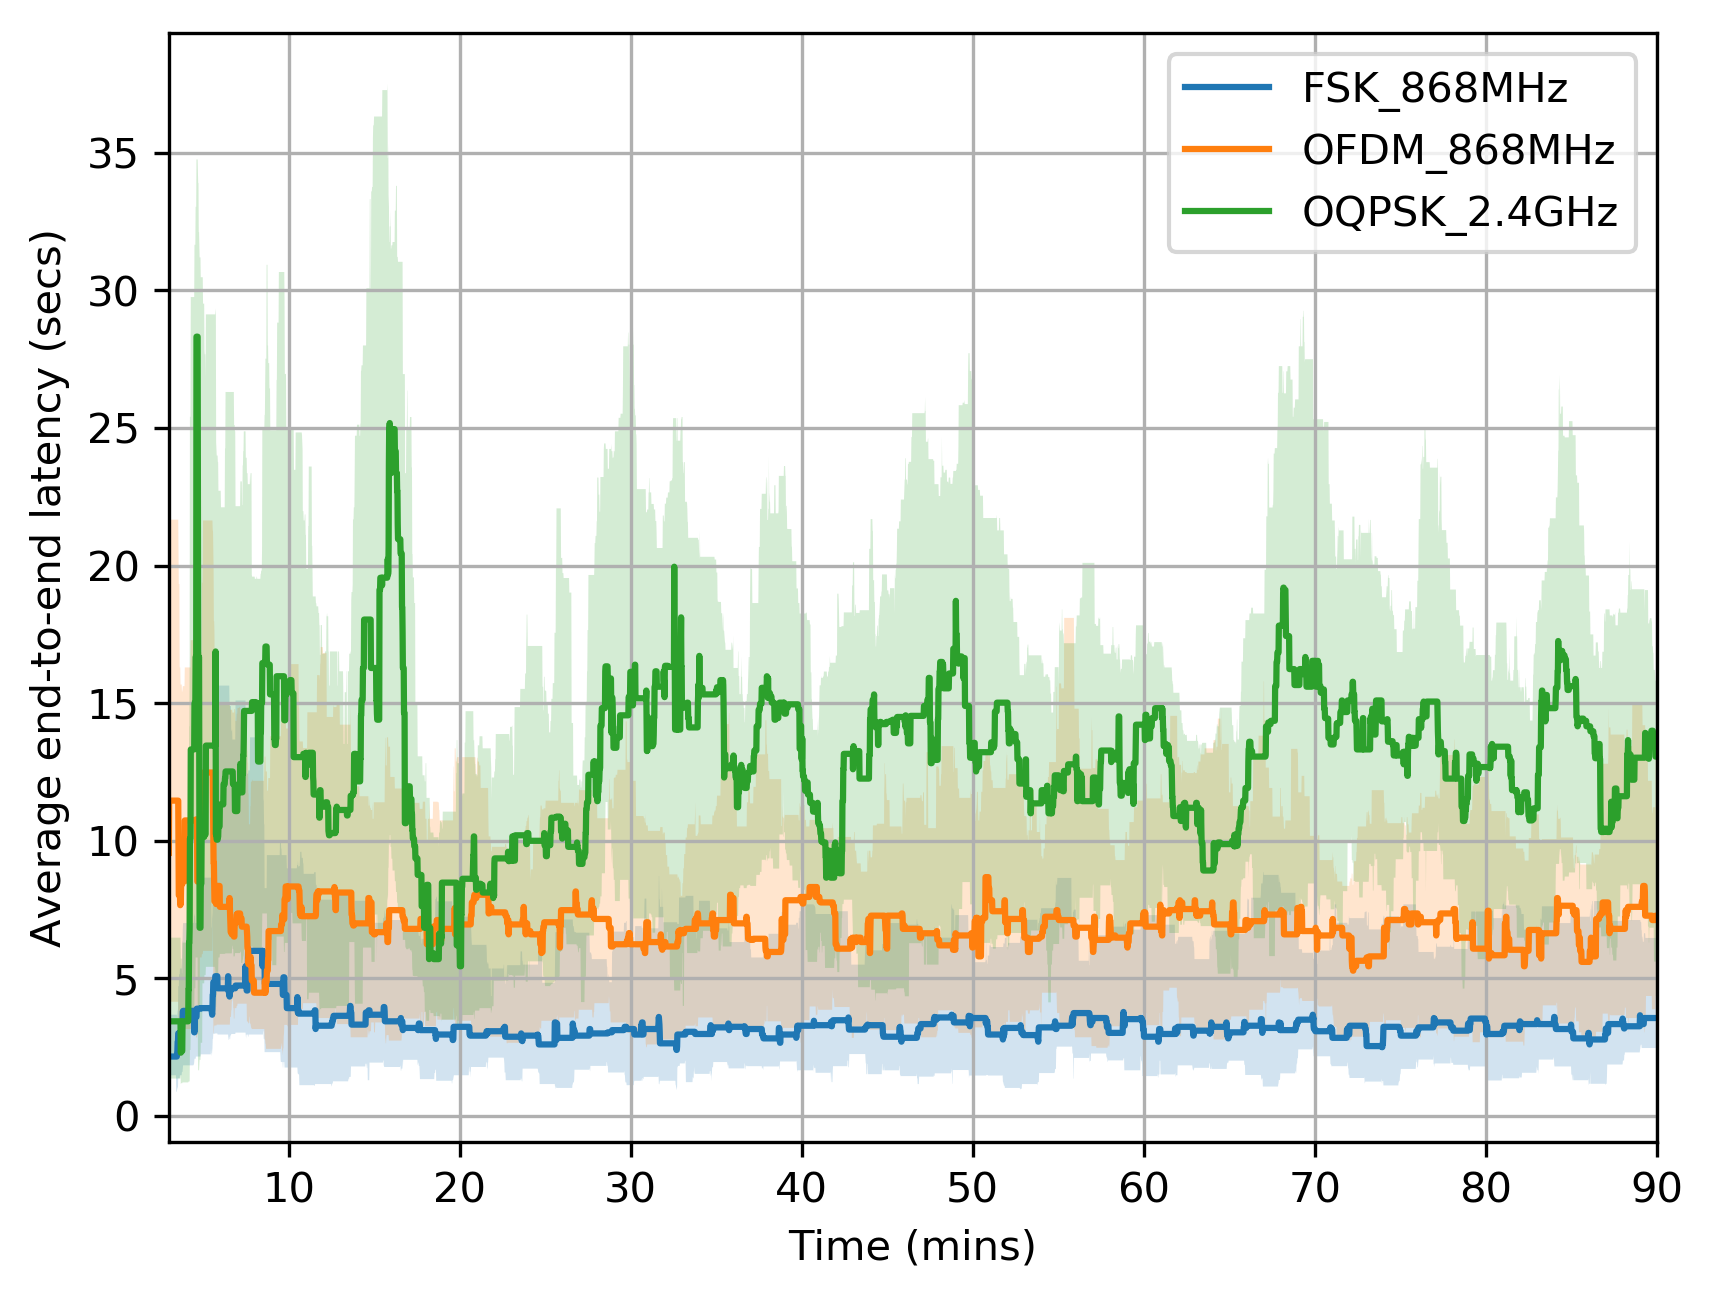
\includegraphics[width=0.90\columnwidth]{avg_latency_plot}
	\caption{Average end-to-end latency. Shaded curves represent the majority of the distribution (interquartile range)}
    \label{fig:avg_latency_plot}
\end{figure}

%------------------------------------------------------------------------------
\subsection{Queue Occupancy}
\label{sec:queue}

% less neighbors does not mean lower packet buffer footprint

Interestingly enough, it seems that there is an inverse correlation between bit-rate and average packet buffer occupancy as seen in Fig.~\ref{fig:avg_bufferSize_plot}. 
In this setting, the packet queue buffer is of size 20 entries. 
However it seems that the peak of the occupancy in either case is during network formations. 
This is slightly surprising because as a node has on average more neighbors in FSK than OFDM/24GHZ (as seen in Fig.~\ref{fig:avg_numNeighbors_plot}), it is expected that there would be more network overhead for neighbor negotiation using sixtop packets; on the contrary, the overall average buffer occupancy is less for FSK. 
This could be explained by the fact that more re-transmissions are needed as bit-rate goes higher, leading to more buffer occupancy ratio on average. 

\begin{figure}
	\centering
	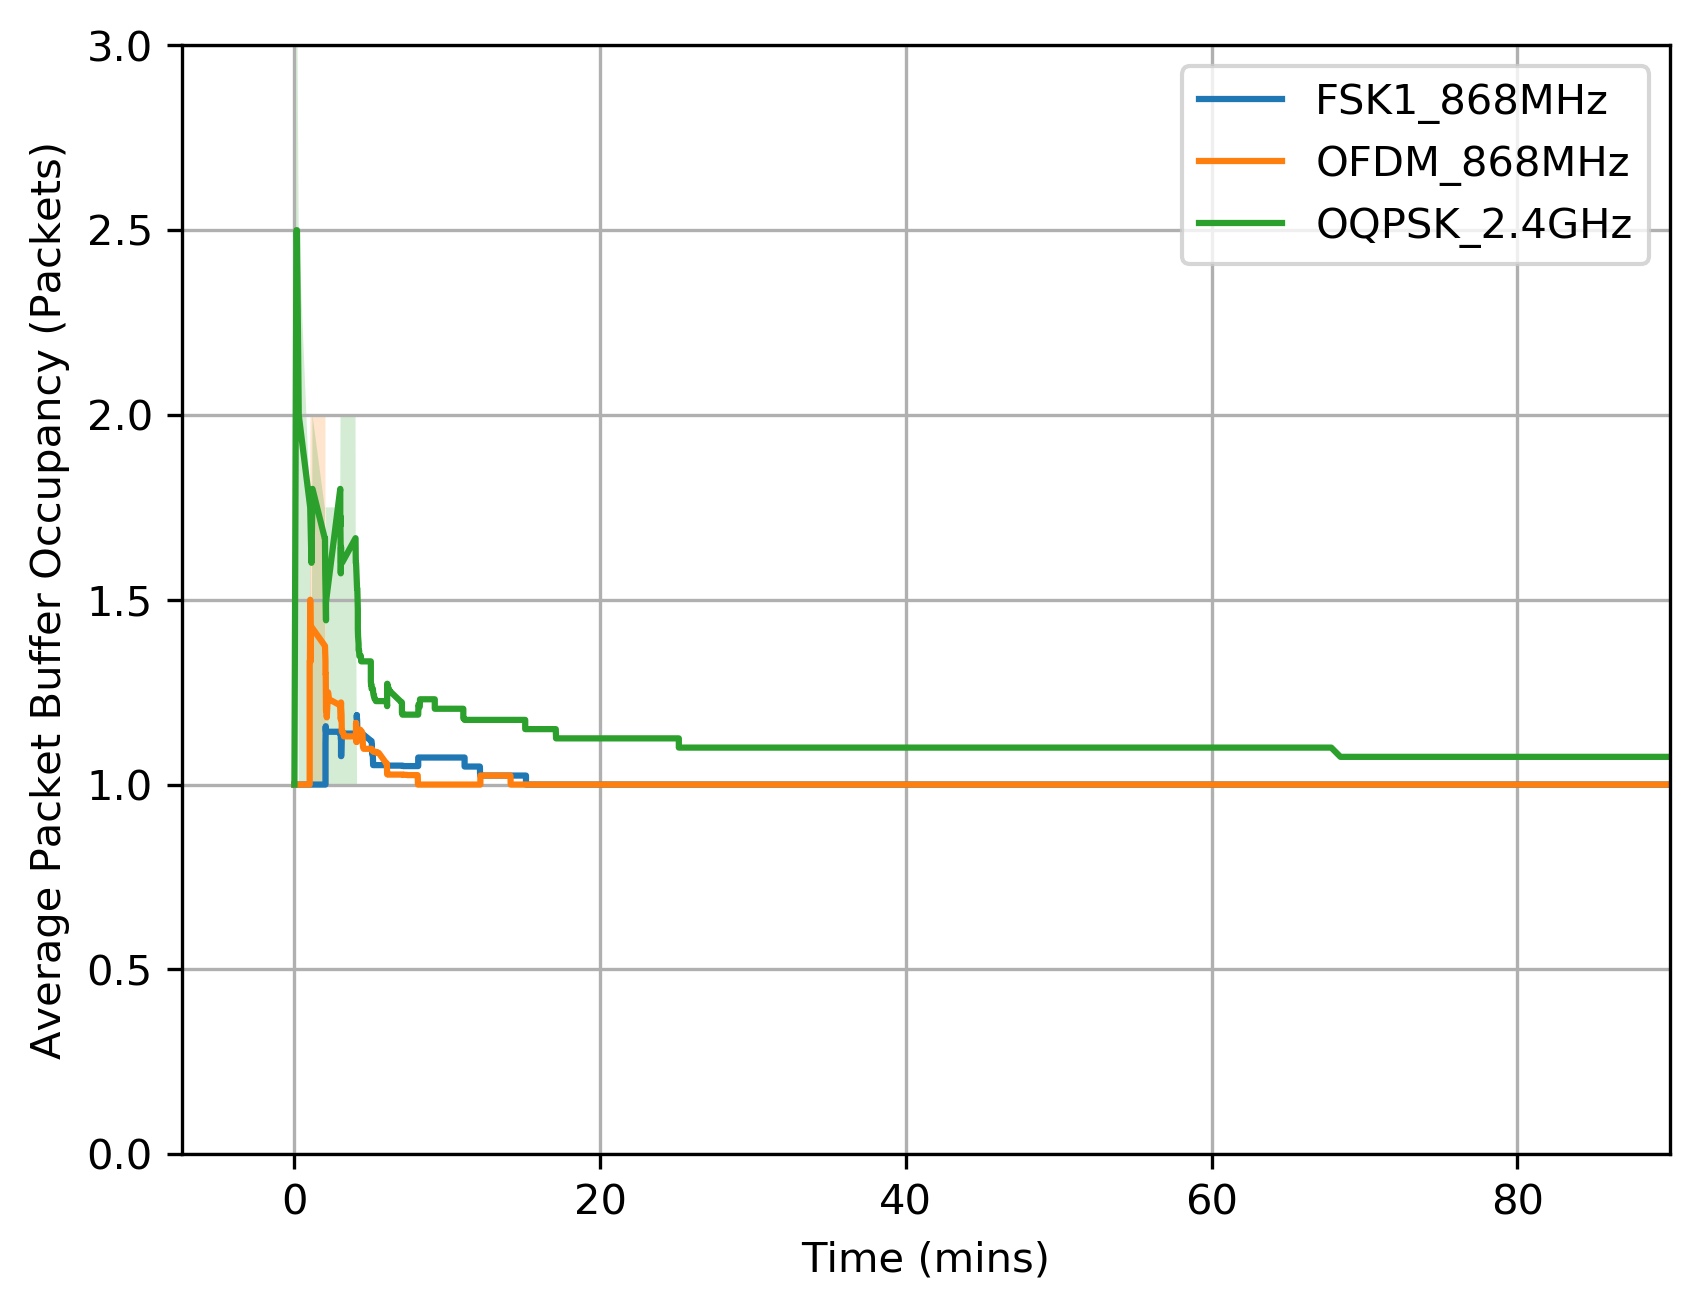
\includegraphics[width=0.90\columnwidth]{avg_bufferSize_plot}
	\caption{Average queue occupancy.}
    \label{fig:avg_bufferSize_plot}
\end{figure}

%------------------------------------------------------------------------------
\subsection{Battery Lifetime}
\label{sec:battery_lifetime}

There is an interesting observation in \ref{fig:avg_avg_dutyCycle_plot} and \ref{fig:avg_avg_dutyCycleTx_plot} which is that the average is skewed towards the third quartile.
This could be explained by the few nodes closer to the DAG root (northern nodes) that relay traffic that is multiple orders of magnitude more than southern nodes. 

\begin{figure}
	\centering
	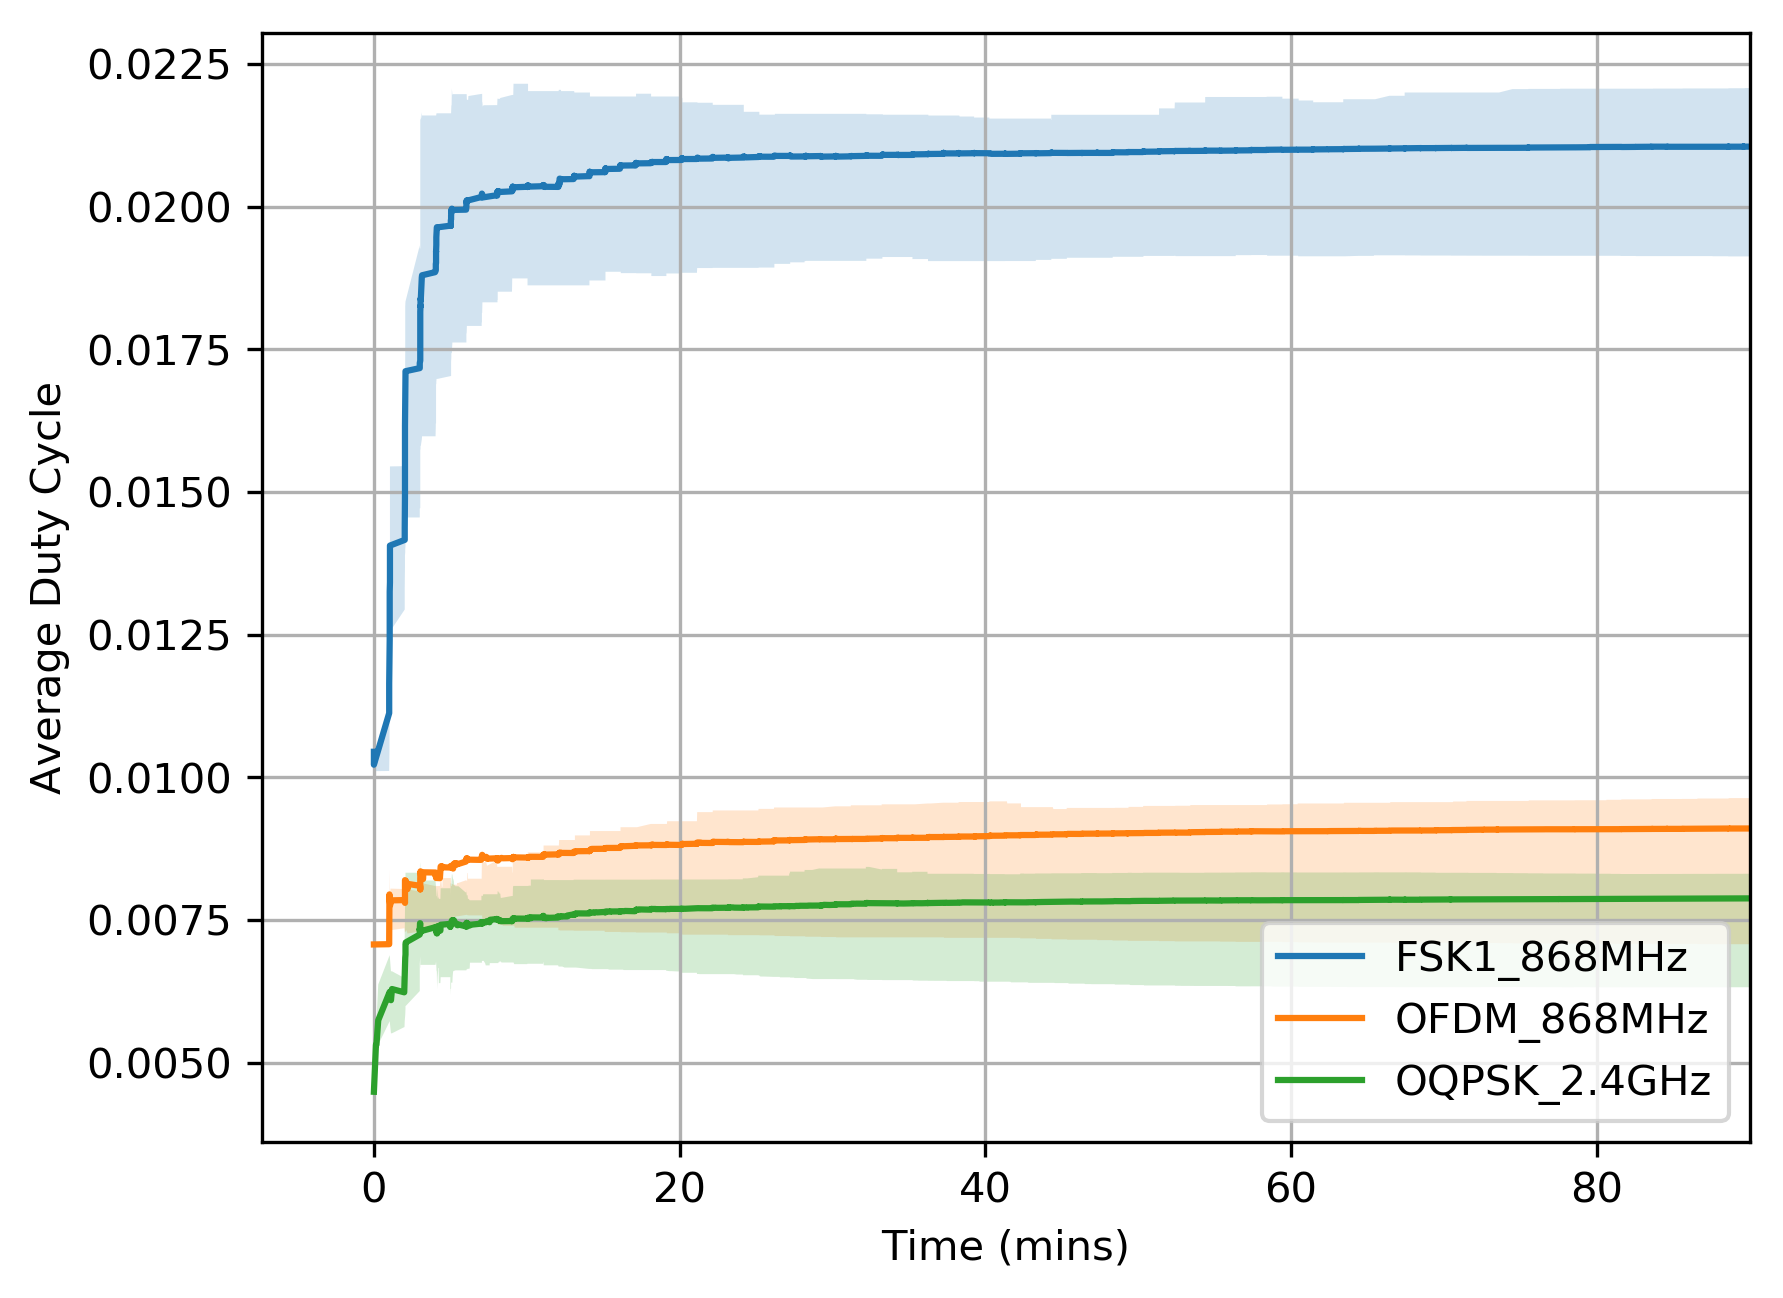
\includegraphics[width=0.90\columnwidth]{avg_avg_dutyCycle_plot}
	\caption{Average duty cycle.Shaded curves represent the majority of the distribution (interquartile range)}
    \label{fig:avg_avg_dutyCycle_plot}
\end{figure}




\mina{We need to discuss how to caclulate the expected battery life. for FSK and OFDM, Tx current is 62 mA but Rx current is 28 mA. For OQPSK in cc2538, Tx current is 24 mA and Rx current is 20 mA.I have the DC\\ measurements for total radio on (not distinguishing tx frm rx (fig 8), and the dc for tx only (fig 9). \\
I propose  to subtract Tx DC from Total Radio on DC, and assume negeligible dataprepare time. Then we calculate the total power consumption accordingly? I did this in the table \ref{tab:energy_table}
}
  


\begin{table*}[t]
 \caption {Battery Life - assuming 2 AA batteries with total 3V and 4.2 wh capacity} \label{tab:energy_table} 
 \begin{center}
\begin{tabular}{lllllllll}
      & Total DC & Tx DC (measured) & \begin{tabular}[c]{@{}l@{}}RX DC\\ (estimated)\end{tabular} & \begin{tabular}[c]{@{}l@{}}Tx Current \\ (mA)\end{tabular} & \begin{tabular}[c]{@{}l@{}}Rx Current\\  (mA)\end{tabular} & \begin{tabular}[c]{@{}l@{}}Tx Power Consuption \\ (wh)\end{tabular} & \begin{tabular}[c]{@{}l@{}}Rx Power Consumption\\  (wh)\end{tabular} & \begin{tabular}[c]{@{}l@{}}Battery lifetime\\  (days)\end{tabular} \\
\fsk   & 0,02     & 0,00225          & 0,01775                                                     & 62                                                         & 28                                                         & 0,186                                                               & 0,084                                                                & 251,4997                                                           \\
\ofdm  & 0,00875  & 0,000375         & 0,008375                                                    & 62                                                         & 28                                                         & 0,186                                                               & 0,084                                                                & 872,3785                                                           \\
\oqpsk & 0,0077   & 0,0005           & 0,0072                                                      & 24                                                         & 20                                                         & 0,072                                                               & 0,06                                                                 & 2607,892                                                          
\end{tabular}
\end{center}
\end{table*}
%------------------------------------------------------------------------------
\subsection{Discussion}
\label{sec:discussion}
\begin{table}[]
 \caption {6TiSCH performance ranking for each setting} \label{tab:summary}
\begin{tabular}{lllllllll}
      & network fomration speed. & energy & latency & buffer effeciency & pdr &  &  &  \\
\fsk   & 1                        & 3      & 1       & 1                 & 1   &  &  &  \\
\ofdm  & 1                        & 2      & 2       & 1                 & 2   &  &  &  \\
\oqpsk & 3                        & 1      & 3       & 2                 & 1   &  &  & 
\end{tabular}
\end{table}


%\begin{figure}
%	\centering
%	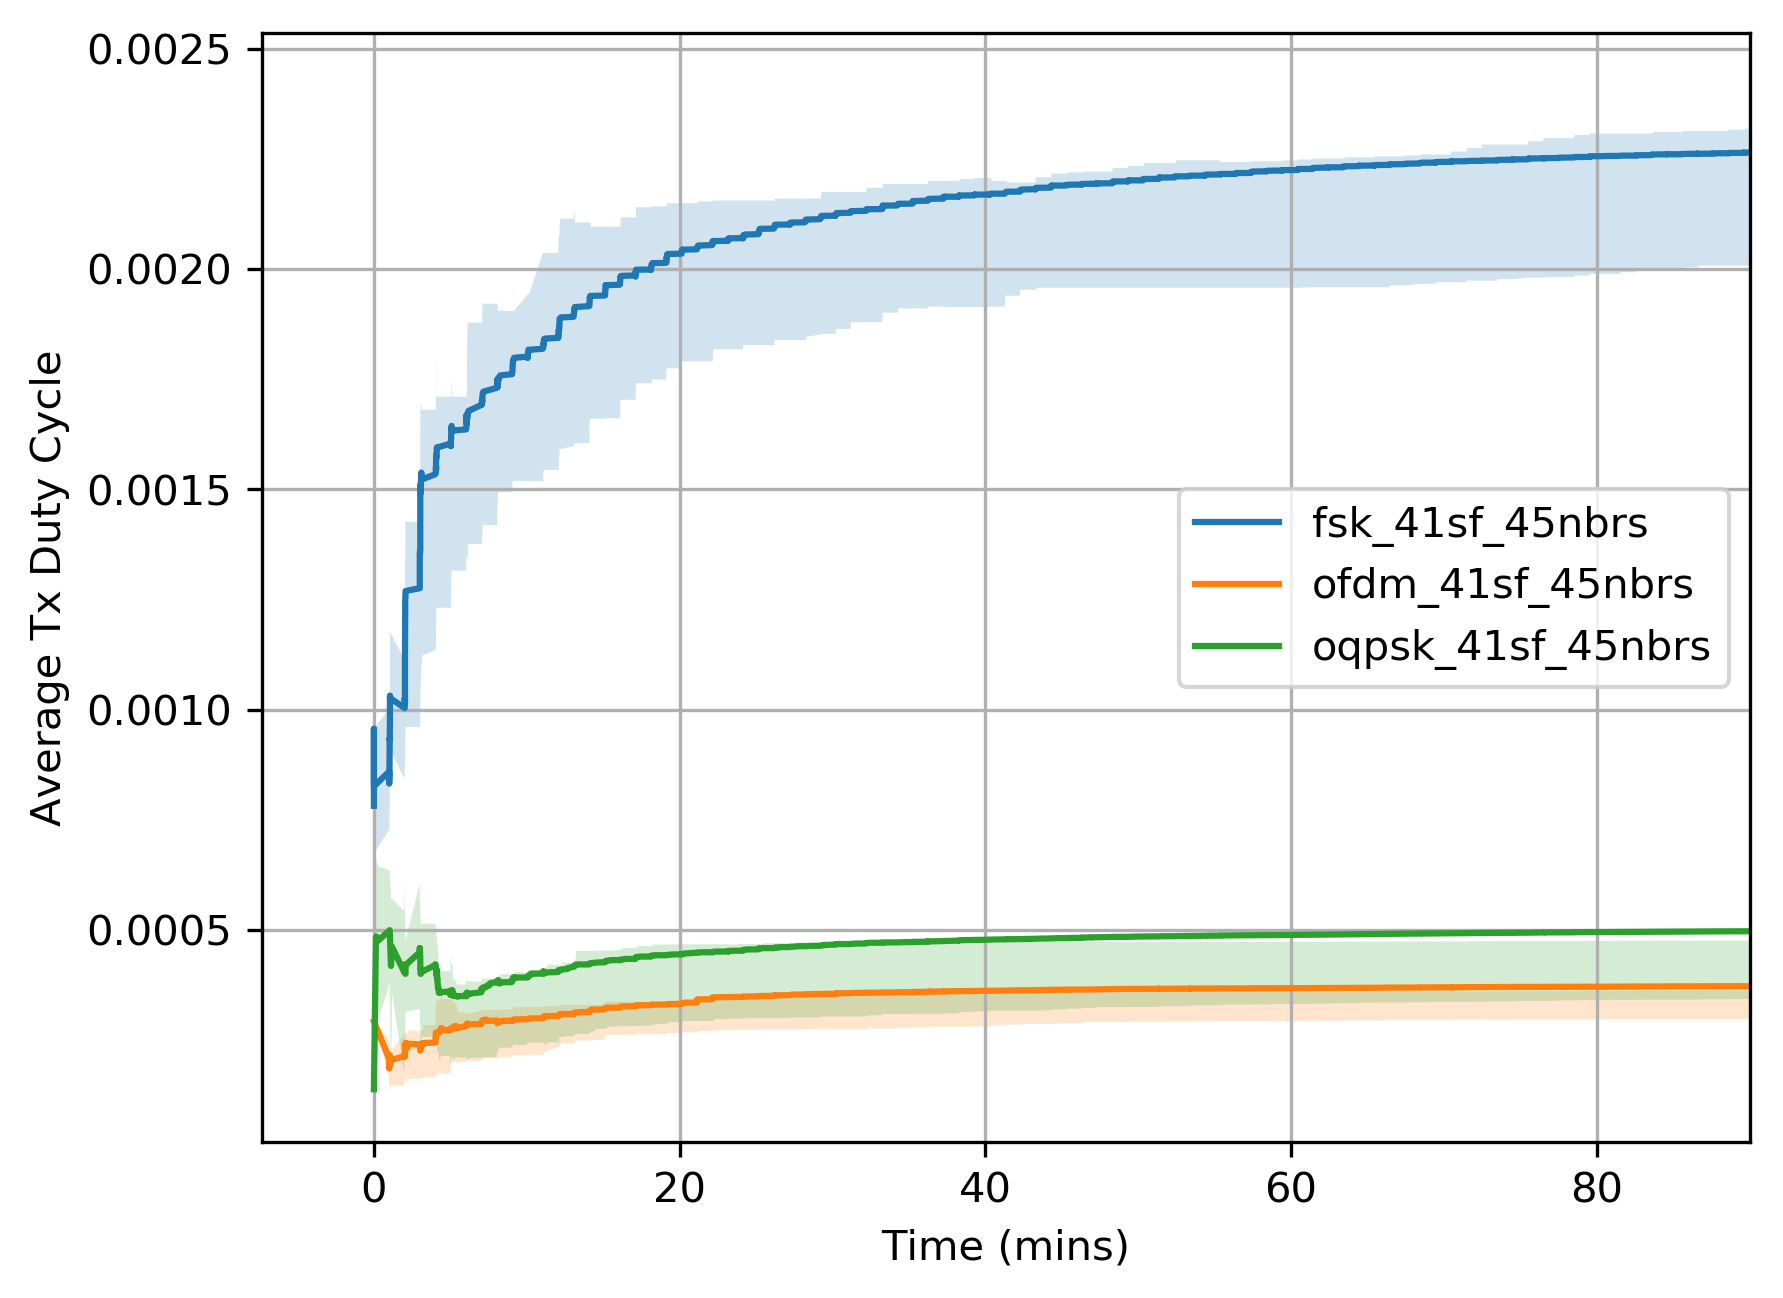
\includegraphics[width=0.90\columnwidth]{avg_avg_dutyCycleTx_plot}
%	\caption{Average transmission duty cycle}
%   \label{fig:avg_avg_dutyCycleTx_plot}
%\end{figure}

%------------------------------------------------------------------------------


%==============================================================================


\end{document}

%==============================================================================
\section{Summary}

The experiments evaluate the impact of utilization of different radio access technologies at the physical layer of the 6TiSCH stack.
\begin{itemize}
    \item FSK 1 in the subghz band
    \item OFDM 1 MCS3 in the subghz band
    \item OQPSK in the 2.4 GHz band
\end{itemize}

The stack performance is evaluated at a end-to-end looking at  KPIs relevant to an SLA for a critical infrastructure, namely:
\begin{itemize}
    \item Network formation time: defined as CDF of time to first packet from all connected motes within a 30 minute time span.
    \item Reliability: defined in terms of PDR
    \item Quality of Service: defined as traffic latency
    \item Battery lifetime: expected lifetime with a power supply of 2 AA batteries.
    \item Resilience: defined as combination of two metrics: PDR of connected motes and ratio of disconnected motes (i.e. motes that were once connected) after sudden total failure of 10\% of the motes in the network (fixed set). 
\end{itemize}
    
Furthermore, the stack performance on top of each radio is evaluated at system-level for the following scenarios:
\begin{itemize}
    \item Increased traffic demand (by 300\%)
    \item Lower Network size and density (by 50\%)
\end{itemize}

%==============================================================================
\section{Draft outline}

\begin{enumerate}
    \item We explore the performance of the 6TiSCH stack in heterogeneous radio settings and we comment on the following aspects of the stack performance: network formation, reliability, quality of service, and power consumption. We observe the following. \item FSK leads to faster network formation (section \ref{sec:network_formation}). 
    \item However, FSK , as robust as it is, can lead to overall lower end-to-end reliability , which is contrary to the case of OFDM (section \ref{sec:reliability}) 
    \item Despite the lower PDR of the 6TiSCH stack in top of FSK, it shows much more end-to-end stable latency. (section \ref{sec:quality_of_service})
    \item Shorter range radios , even though they consume less energy in principle, they have a side effect as they can lead to the occupancy of the packet memory buffer due to consistent re-transmissions. This could risk reaching buffer overflow as network traffic increases. (section \ref{sec:quality_of_service})
    \item Furthermore, higher reliability of OFDM does not mean higher resilience. 
    Even though OFDM shows 99.6-100\% PDR on average compared to 99.0-99.5\% average PDR for FSK, FSK shows the best resilience in terms of PDR maintenance.  
    FSK result into a higher network degree which risks reaching limits of allocated memory buffers allocated for storage of neighbor information (section \ref{sec:resilience})
    \item Despite the advantages of FSK for end-to-end latency and network formation speed, its power consumption present a significant drawback. Also, despite the higher bitrate of OFDM compared to OQPSK, it ends up consuming similar duty cycles (b/c of re-transmissions?) (section \ref{sec:battery_lifetime})
\end{enumerate}

\begin{figure}
	\centering
	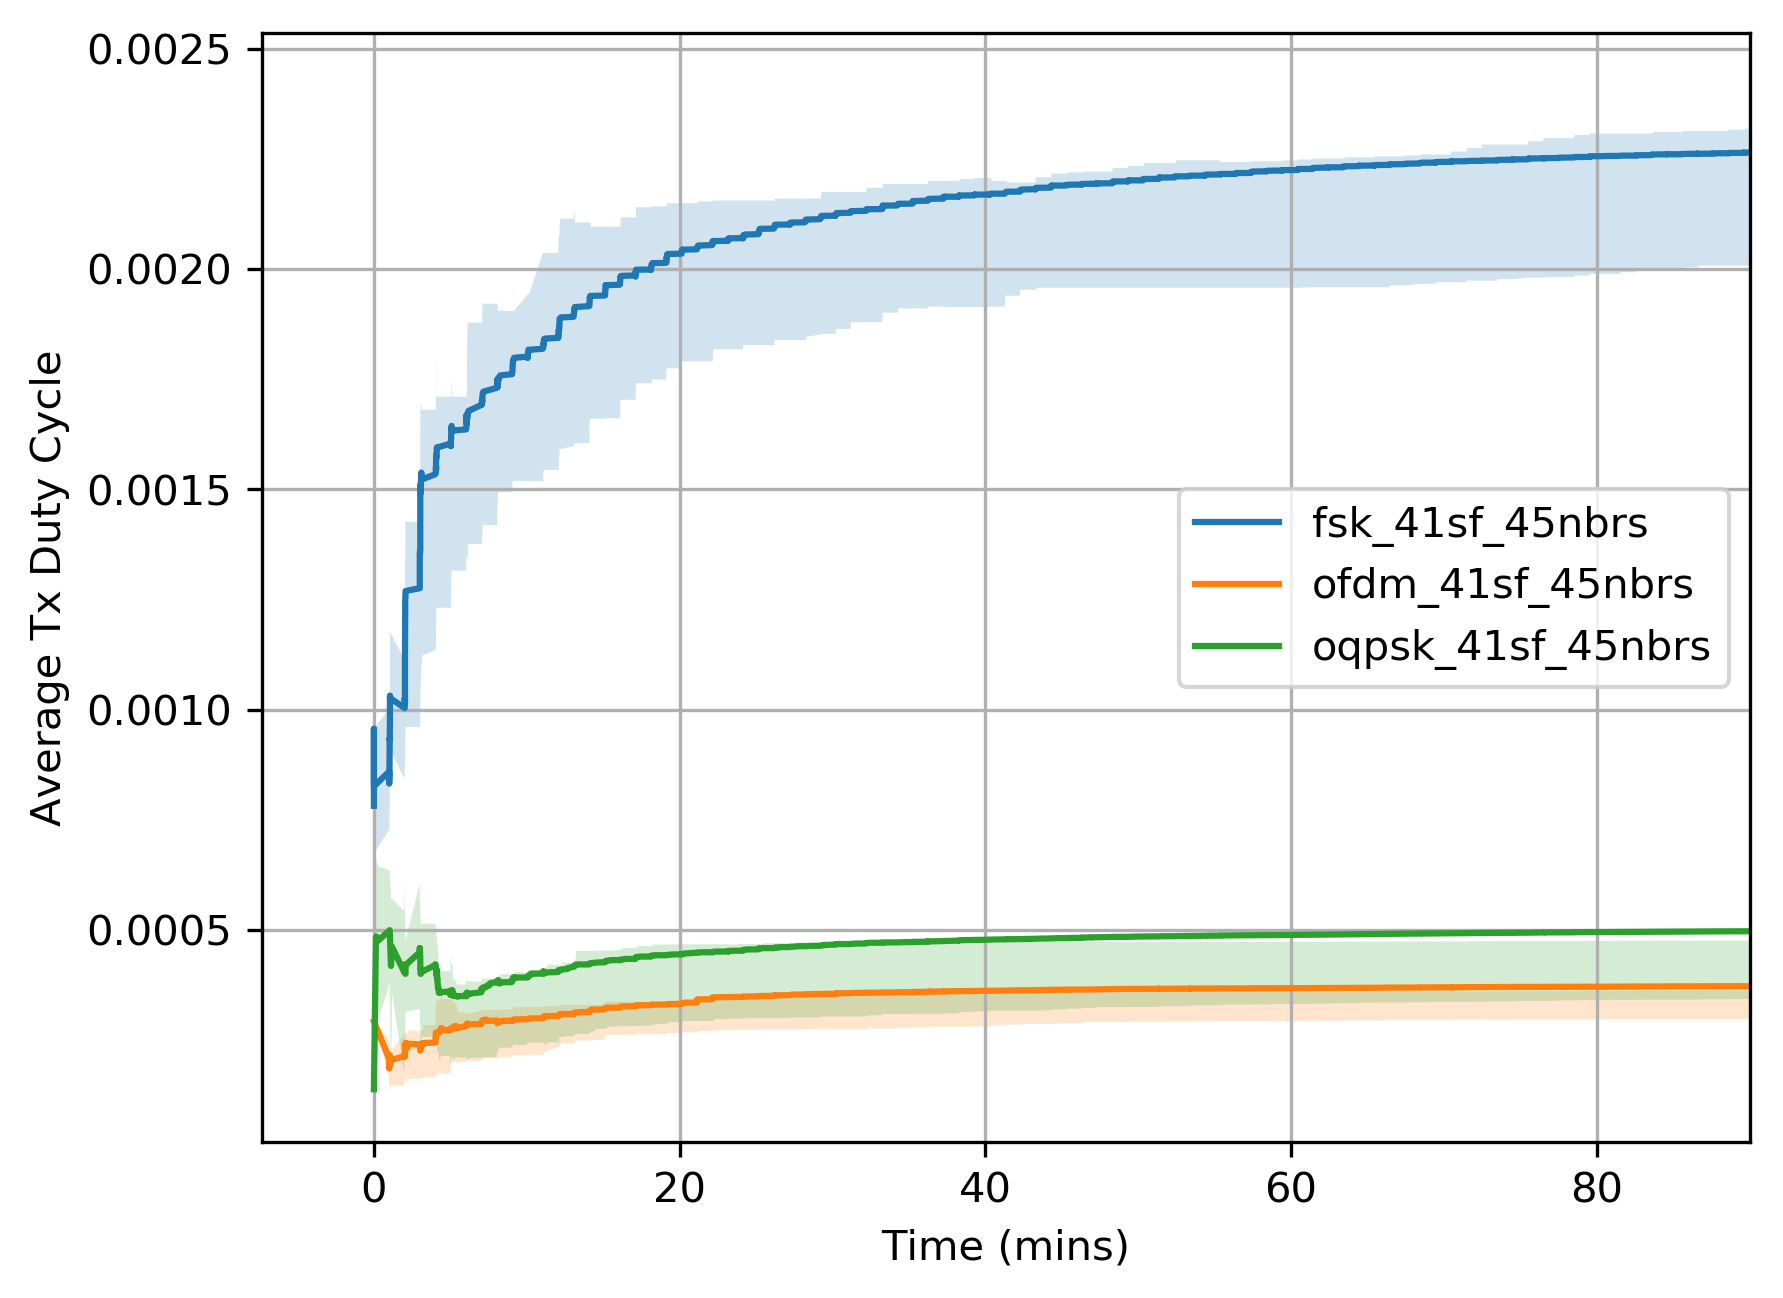
\includegraphics[width=0.90\columnwidth]{avg_avg_dutyCycleTx_plot}
	\caption{Average duty cycle. Shaded curves represent the majority of the distribution (interquartile range).}
    \label{fig:avg_avg_dutyCycleTx_plot}
\end{figure}